\documentclass[11pt]{article}
\usepackage{amsmath}
\usepackage{amssymb}
\usepackage{graphicx}
\usepackage{float}
\usepackage{subcaption}
\usepackage{fancyhdr}
\usepackage{enumerate}
\usepackage{titlesec}
\usepackage{listings}
\usepackage[colorlinks=true,urlcolor=blue]{hyperref}
\titlespacing{\subsubsection}{0pt}{0pt}{0pt}

% No page numbers
%\pagenumbering{gobble}

% INFORMATION SHEET (DO NOT EDIT THIS PART) ---------------------------------------------
\newcommand{\addinformationsheet}{
\clearpage
\thispagestyle{empty}
\begin{center}
\LARGE{\bf \textsf{Information sheet\\CS224W: Machine Learning with Graphs}} \\*[4ex]
\end{center}
\vfill
\textbf{Assignment Submission } Fill in and include this information sheet with each of your assignments.  This page should be the last page of your submission.  Assignments are due at 11:59pm and are always due on a Thursday.  All students (SCPD and non-SCPD) must submit their homework via GradeScope (\url{http://www.gradescope.com}). Students can typeset or scan their homework. Make sure that you answer each (sub-)question on a separate page. That is, one answer per page regardless of the answer length. Students also need to upload their code on Gradescope. Make sure to upload all of your code as .py files.
\\
\\
\textbf{Late Homework Policy } Each student will have a total of {\em two} late periods. {\em Homework are due on Thursdays at 11:59pm PT and one late period expires on the following Monday at 11:59pm PT}.  Only one late period may be used for an assignment.  Any homework received after 11:59pm PT on the Monday following the homework due date will receive no credit.  Once these late periods are exhausted, any assignments turned in late will receive no credit.
\\
\\
\textbf{Honor Code } We strongly encourage students to form study groups. Students may discuss and work on homework problems in groups. However, each student must write down their solutions independently, i.e., each student must understand the solution well enough in order to reconstruct it by him/herself.  Students should clearly mention the names of all the other students who were part of their discussion group. Using code or solutions obtained from the web (GitHub/Google/previous year's solutions etc.) is considered an honor code violation. We check all the submissions for plagiarism. We take the honor code very seriously and expect students to do the same. 
\vfill
}

% MARGINS (DO NOT EDIT) ---------------------------------------------
\oddsidemargin  0.25in \evensidemargin 0.25in \topmargin -0.5in
\headheight 0in \headsep 0.1in
\textwidth  6.5in \textheight 9in
\parskip 1.25ex  \parindent 0ex \footskip 20pt
% ---------------------------------------------------------------------------------

% HEADER (DO NOT EDIT) -----------------------------------------------
\newcommand{\problemnumber}{0}
\newcommand{\myname}{name}
\newfont{\myfont}{cmssbx10 scaled 1000}
\pagestyle{fancy}
\fancyhead{}
\fancyhead[L]{\myfont Question \problemnumber, Homework 3, CS224W}
%\fancyhead[R]{\bssnine \myname}
\newcommand{\newquestion}[1]{
\clearpage % page break and flush floats
\renewcommand{\problemnumber}{#1} % set problem number for header
\phantom{}  % Put something on the page so it shows
}
% ---------------------------------------------------------------------------------


% BEGIN HOMEWORK HERE
\begin{document}


\newquestion{1.1}
\\
Total nodes of email:  265214 \\
IN of 2018 in email:  1 \\
OUT of 2018 in email:  52104 \\
Total nodes of epinions:  75879 \\
IN of 224 in epinions:  56459 \\
OUT of 224 in epinions:  47676 \\
\\
According to the definition, node 2018 of email lies in IN and node 224 of epinions lies in SCC.

\newquestion{1.2}
Plot for email is as below:
\begin{figure}[H]
    \centering
    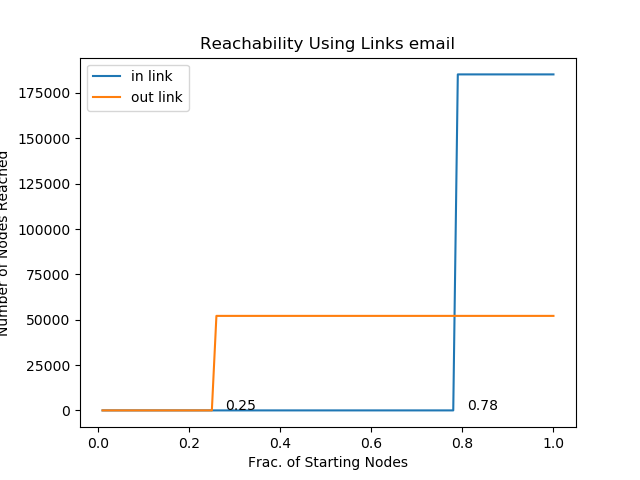
\includegraphics[width=0.50\textwidth]{pic/q1_2_email.png}
\end{figure}
From the picture we can roughly estimate that relative sizes of SCC, IN and OUT are  16.5\%,  58.5\%, 5.5\%.
\\
Plot for epinions is as below:
\begin{figure}[H]
    \centering
    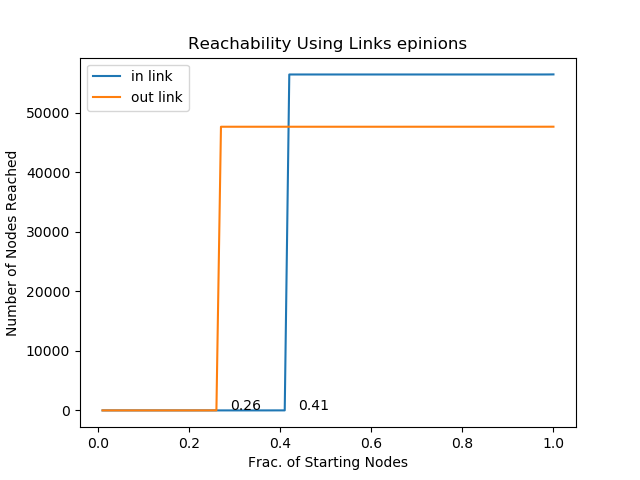
\includegraphics[width=0.50\textwidth]{pic/q1_2_ep.png}
\end{figure}
From the picture we can roughly estimate that relative sizes of SCC, IN and OUT are  43.66\%,  30.34\%, 15.34\%.

\newquestion{1.3}
\\
Firstly, we can use (total\_nodes - MxWcc\_size) and MxScc\_size to calculate the sizes of DISCONNECT and SCC.
Then starting from any node in SCC, do one forward BFS to calculate the size of OUT and one backward BFS to calculate the size of IN.
The left is TENDRILS+TUBES(TT). The results are as follows:
\\
Total nodes of email:  265214 \\
Size of MxWcc in email:  224832 \\
Size of MxScc in email:  34203 \\
Size of IN in email:  151023 \\
Size of OUT in email:  17900 \\
Size of TT in email:  21706 \\
Size of DISCONNECT in email:  40382 \\
\\
Total nodes of epinions:  75879 \\
Size of MxWcc in epinions:  75877 \\
Size of MxScc in epinions:  32223 \\
Size of IN in epinions:  24236 \\
Size of OUT in epinions:  15453 \\
Size of TT in epinions:  3965 \\
Size of DISCONNECT in epinions:  2 \\

\newquestion{1.4}
The sampled probabiltiy plots are as follows:
\begin{figure}[H]
    \centering
    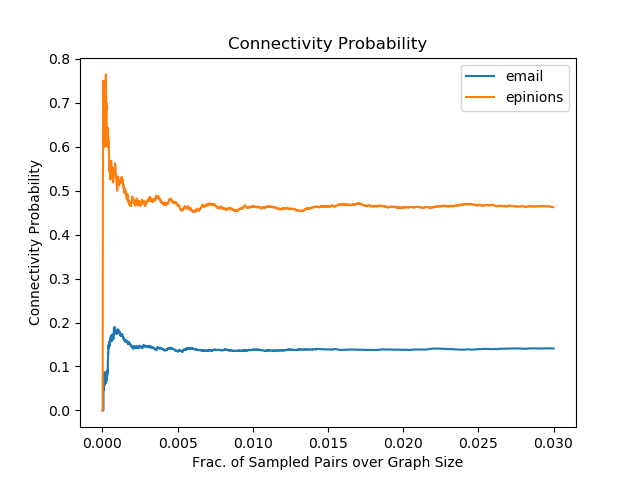
\includegraphics[width=0.50\textwidth]{pic/q1_con.png}
\end{figure}
We can see that both of email and epinions converge to 14\% and 46\%. \\\\
If we neglect the other parts, the probabiltiy will be converged to
$$
    p = \frac{size_{IN}+size_{SCC}}{size_{IN}+size_{SCC}+size_{OUT}}*\frac{size_{OUT}+size_{SCC}}{size_{IN}+size_{SCC}+size_{OUT}}
$$
which is higher than (23\%, 52\% respectively for email and epinions), since other parts still take up a certain number of percentage of the graph.

\newquestion{2.1}
Yes. We can compute the probabilties for these guys. Just set the restart point of random walk to be the points in
the corresponding teleport set (uniformly or according to the weights).


\newquestion{2.2}
As long as the choosing of restart points of the random walk is uniform, we can compute personalized pagerank vectors of
whose teleport set can be added (or minus) by others in $V$.


\newquestion{2.3}
The calculation procedure can be written as:
\begin{equation*}
    \begin{aligned}
        r & = M r                                                     \\
          & = \beta M r + \frac{1-\beta}{N} \mathrm{1} \mathrm{1}^T r \\
    \end{aligned}
\end{equation*}

For every $r_i$ in the left, the right part $\frac{1-\beta}{N} \mathrm{1} \mathrm{1}^T r$ contributes $\frac{1-\beta}{N} \Sigma_i r_i$,
as $\Sigma_i r_i = 1$, then we have$$r = \beta M r + \frac{1-\beta}{N} \mathrm{1}$$.

\newquestion{3.1}
Sadly, to the best of my knowledge, my implementation tells that \\
In graph 1, candidate B wins by 162 votes \\
In graph 2, candidate B wins by 332 votes \\

\newquestion{3.2}
Results are \\
On graph 1, the minimum amount you can spend to win is 7000 \\
On graph 2, the minimum amount you can spend to win is 1000 \\
\begin{figure}[H]
    \centering
    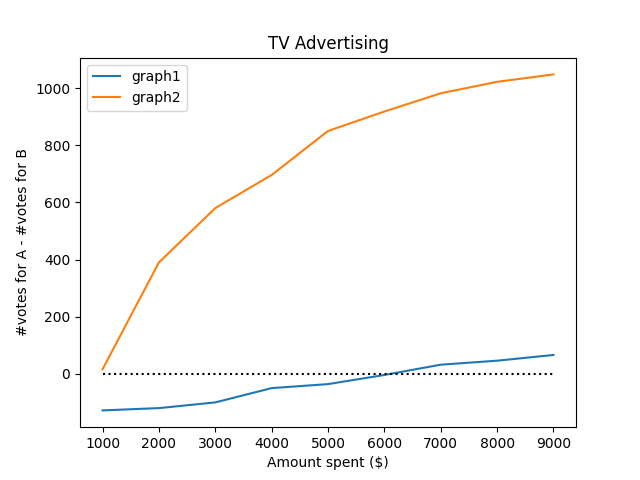
\includegraphics[width=0.50\textwidth]{pic/q3_adv.png}
\end{figure}


\newquestion{3.3}
Results are \\
On graph 1, the minimum amount you can spend to win is \textit{INF} \\
On graph 2, the minimum amount you can spend to win is 6000 \\
\begin{figure}[H]
    \centering
    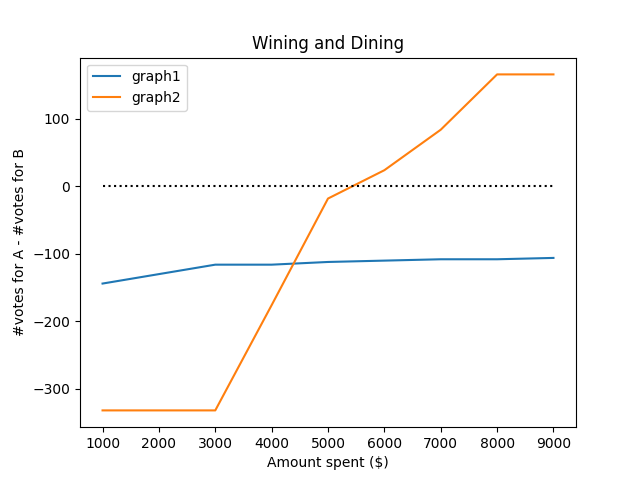
\includegraphics[width=0.50\textwidth]{pic/q3_dining.png}
\end{figure}

\newquestion{3.4}
The log-log distribution is like below
\begin{figure}[H]
    \centering
    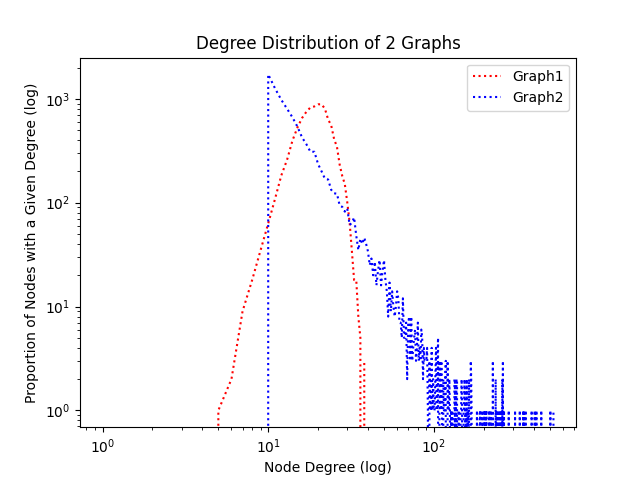
\includegraphics[width=0.50\textwidth]{pic/q3_dist.png}
\end{figure}
We can see that Graph2 have more nodes with high degrees, so it's effective to invite high rollers in order to win vote.
However, in case of advertising, changing nodes with less neigbors may bring limited contribution to win the vote.


\newquestion{4.1}
Take the below graph as an example:
\begin{figure}[H]
    \centering
    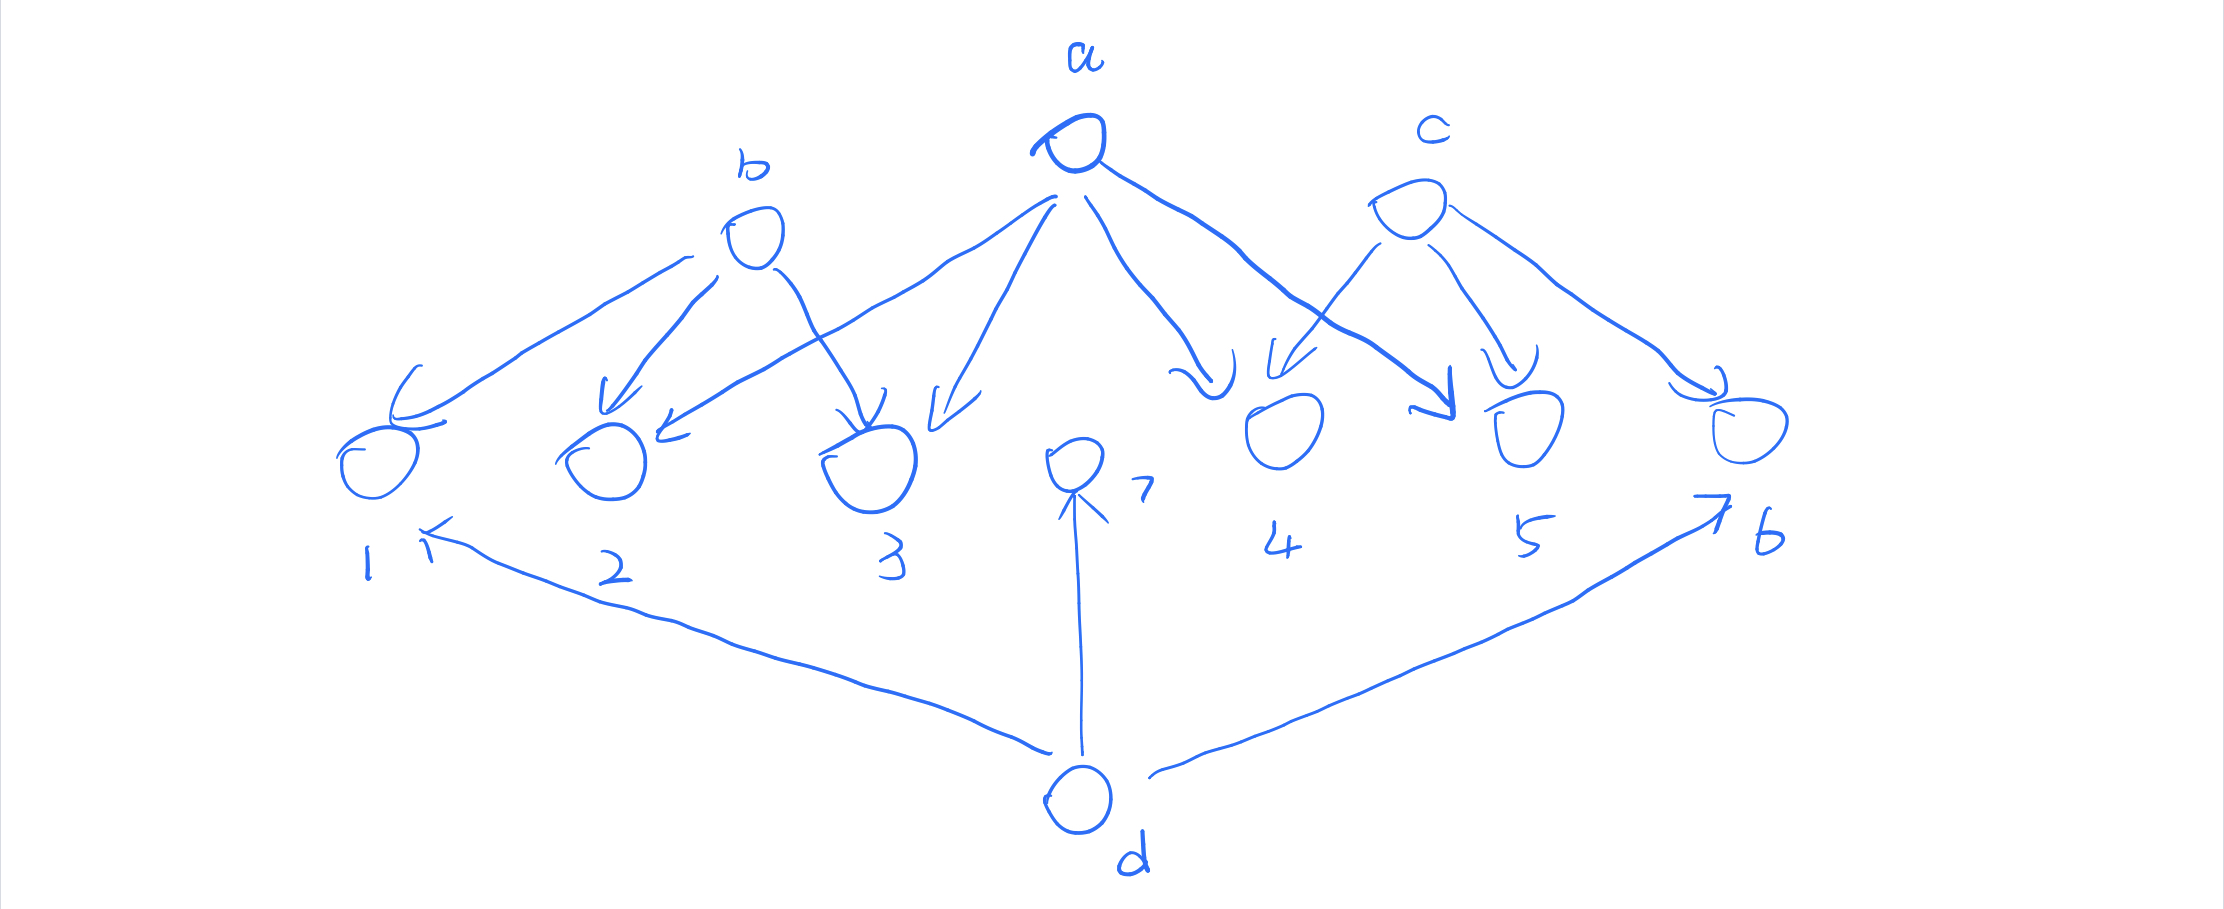
\includegraphics[width=0.50\textwidth]{pic/q4_example.PNG}
\end{figure}
when $k=2$, $|X_u|=|\{b,1\}|=7$, $S=\{a,b\}$, $T=\{b,c\}$ and $f(T)=|\{b,1,2,3,c,4,5,6\}|=8$.

\newquestion{4.2}
Here is the graph, we have $T=\{b,c,d\}$ and $S=\{a,b,c\}$,
where each $a,b,c,d$ connect with $3k$ nodes, and $Nbr(a)$ shares different $k$ nodes with $Nbr(b),Nbr(c),Nbr(d)$.
Then we have $f(T)=9k$ and $f(S)=7k+1$, let $0.8f(T)=f(S)$, we have $k=20$.


\newquestion{4.3}
$$|X_u|=1$$

\newquestion{4.4}
\begin{figure}[H]
    \centering
    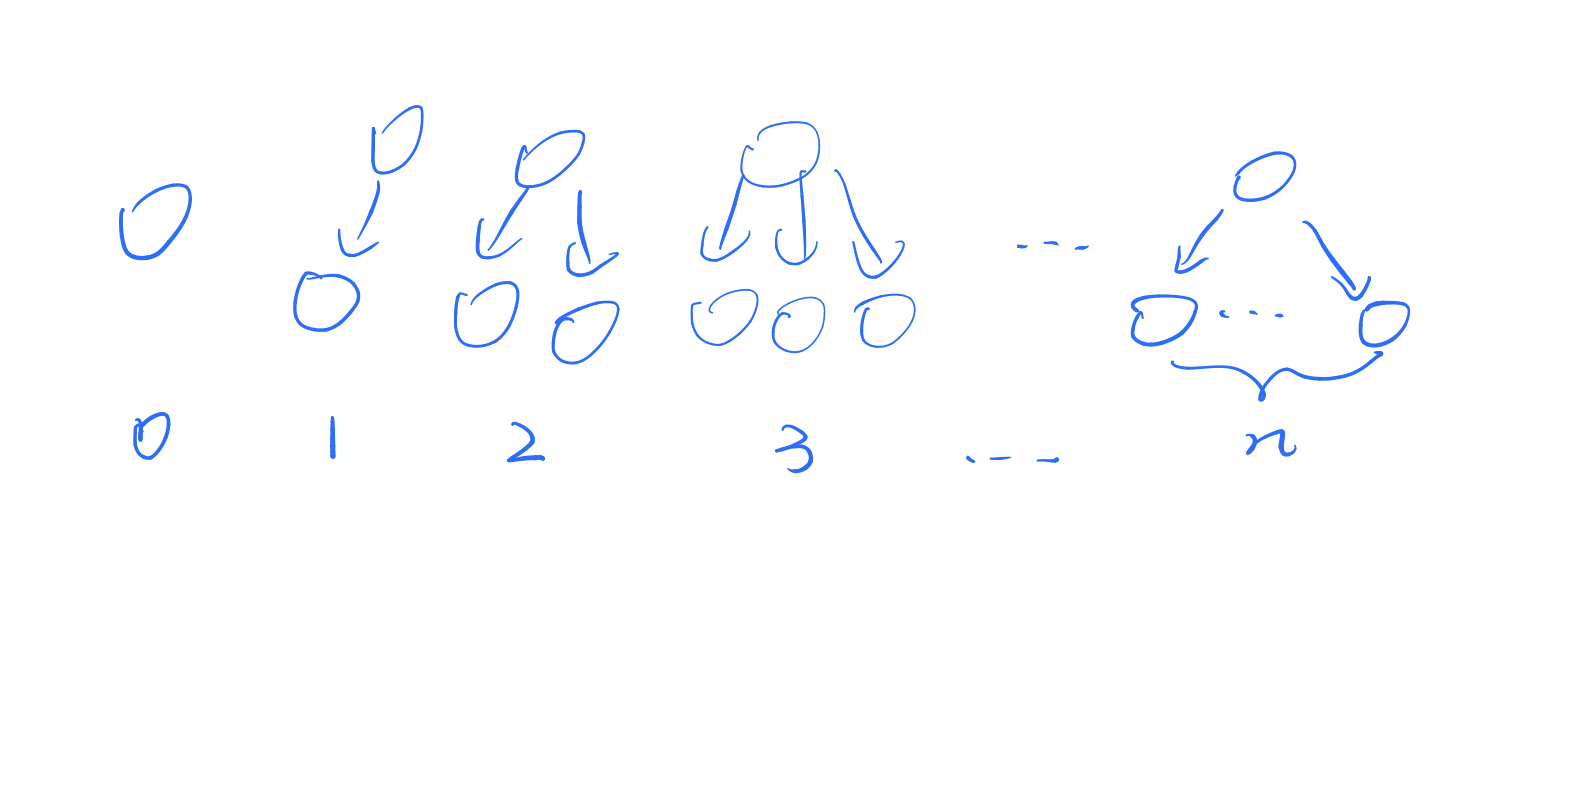
\includegraphics[width=0.50\textwidth]{pic/q4_example2.PNG}
\end{figure}

% Information sheet
% Fill out the information below (this should be the last page of your assignment)
\addinformationsheet
\vfill

{\Large
    \textbf{Your name:} \hrulefill  % Put your name here
    \\
    \\
    \textbf{Email:} \underline{\hspace*{7cm}}  % Put your e-mail here
    \textbf{SUID:} \hrulefill  % Put your student ID here
    \\*[2ex]
}
Discussion Group: \hrulefill   % List your study group here
\\
\vfill\vfill
I acknowledge and accept the Honor Code.\\*[3ex]
\bigskip
\textit{(Signed)}
\hrulefill   % Replace this line with your initials
\vfill






\end{document}